% \documentclass[10pt, twocolumn, a4paper]{article}
\documentclass[12pt,a4paper]{article}

\usepackage[backend=biber, style=ieee]{biblatex}                        % To include the bibliography
\usepackage[left=2cm, right=2cm, top=2.5cm, bottom=2.5cm]{geometry}     % To set the margins
\usepackage[noend]{algpseudocode}
\usepackage[table]{xcolor}                                              % For coloring cells

\usepackage{algorithm}                                                  % To include algorithms
\usepackage{amsfonts}                                                   % To include math fonts:ToggleTerm direction=float
\usepackage{amsmath}                                                    % To include Mathematic symbols
\usepackage{authblk}                                                    % To format author affiliations
\usepackage{caption}                                                    % For caption spacing
\usepackage{float}                                                      % To place figures where you want them
\usepackage{graphicx}                                                   % To include images
\usepackage{hyperref}                                                   % To include hyperlinks
\usepackage{lipsum}                                                     % TODO: remove this
\usepackage{listings}                                                   % To include code
\usepackage{tabularx}                                                   % For equal-width columns
\usepackage{tcolorbox}                                                  % To make colored boxes
\usepackage{tikz}                                                       % To draw graphs
\usepackage{titlesec}                                                   % To format section titles
\usepackage{xcolor}                                                     % To define colors

\usetikzlibrary{graphs,graphs.standard}
\usetikzlibrary{positioning}

\addbibresource{./references.bib}

% Esto es para poder hacer cajitas de código con el fondo gris
\lstset{
    language=C++,
    basicstyle=\ttfamily\small,
    keywordstyle=\color{blue}\bfseries,
    stringstyle=\color{green!60!black},
    commentstyle=\color{gray},
    backgroundcolor=\color{gray!05},
    frame=single,
    numbers=left,
    numberstyle=\small,
    stepnumber=1,
    numbersep=10pt,
    tabsize=2,
    showstringspaces=false,
    captionpos=b,
}

% Para poder hacer flechas
\usetikzlibrary{shapes, arrows}

% Sección de definiciones
\titleformat{\section}{\Large\bfseries}{\thesection}{1em}{}
\titleformat{\subsection}{\large\bfseries}{\thesubsection}{1em}{}

% Caja de colores
\definecolor{mint}{RGB}{202,251,202}
\definecolor{yellow}{RGB}{255,255,202}
\definecolor{red}{RGB}{255,202,202}

% Variables globales
\newcommand{\currentsemester}{Segundo Semestre}
\newcommand{\currentyear}{2025}


\begin{document}

\begin{center}
    \LARGE\textbf{Programación Paralela} \\
    \Large{Teórica 02 - Introducción a CUDA} \\
    \normalsize{\currentsemester, \currentyear} \\
    \vspace{1em}
    \hrule
\end{center}

\setcounter{section}{2}

\subsection{Introducción}

Como dijimos en la práctica anterior, la computación paralela es una técnica que permite realizar cálculos de manera
simultánea en múltiples procesadores. Para los ejercicios vamos a utilizar CUDA C que nos permite escribir programas
paralelos escalables en sistemas donde conviven tanto CPUs como GPUs. \textbf{En este tipo de sistemas donde hay
porciones de código que pueden ejecutarse en paralelo, pero que están gobernadas por un código secuencial que corre en
la CPU, los llamaremos \textit{sistemas heterogéneos}}. CUDA extiende el lenguaje de programación C con una sintaxis
mínima que permite tener código secuencial, gobernado por la CPU, y código que puede ser ejecutado en paralelo en GPUs.

Cuando en el software moderno las aplicaciones se ejecutan \textit{lento}, el problema usualmente suele ser que hay
demasiados datos para ser procesados. Por ejemplo en el procesamiento de imágenes o videos, la simulación de dinámica de
fluidos, el manejo de sistemas complejos como (líneas aéreas), o incluso cosas mucho más sencillas como convertir una
imagen de pixels a escala de grises. Estas tareas se pueden fraccionar en tareas más pequeñas que pueden ser ejecutadas
de manera independiente y paralela.

\begin{tcolorbox}[colback=mint,colframe=yellow!75!black,arc=0pt,outer arc=0pt]
  \textbf{Paralelismo de tareas vs. paralelismo de datos} \\

  El paralelismo de tareas, se refiere a la ejecución de múltiples tareas (no necesariamente las mismas) al mismo tiempo.
  Mientras que el paralelismo de datos, se refiere a la ejecución de la misma tarea con datos diferentes al mismo tiempo.
\end{tcolorbox}

\subsubsection{Estructura de un programa en CUDA C}

La estructura de un programa en CUDA C es similar a un programa en C, lo que refleja su naturaleza heterogénea donde
existe un \textit{host} (CPU) y uno o más \textit{devices} (GPUs) en la computadora. El código fuente CUDA tiene una
mezcla de ambos códigos, uno que se ejecuta en el host, y otro en los devices. Por defecto, todo el código se ejecuta en
el host, aunque vamos a declarar funciones de una forma especial para que puedan ser corridas en los \textit{devices}.

El código con estas extensiones de CUDA tiene que ser compilado con el compilador de NVIDIA, \texttt{nvcc}, que es un
wrapper para el compilador de C, \texttt{gcc}. El compilador de NVIDIA se encarga de: separar el código que se ejecuta en
el host, separar el código que se ejecuta en el device, y de compilarlo con el compilador de C. \textbf{El código
identificado con las \textit{keywords} (palabras reservadas) de CUDA para las funciones paralelas se denominan
\textit{kernels}}. Estos kernels son funciones que están asociadas a estructuras de datos y que van a ser ejecutadas en
paralelo por GPUs. En las situaciones donde no haya una GPU disponible, el código de todas formas se ejecutará en una
CPU (uno podría incluso ejecuar el kernel en una CPU utilizando herramientas como MCUDA) \cite{sutter2005}.

La ejecuciónm de un programa en CUDA se ilustra en la Figura \ref{fig:execution_cuda}, la ejecución comienza con el
código del host (CPU) y cuando se llama a una función kernel (código paralelo del dispositivo) es ejecutada por un gran
número de threads en un dispositivo. Todos los threads que son generados por un kernel son colectivamente llamados un
\textit{grid}. Estos threads son el vehículo principal de la ejecución paralela en una plataforma CUDA. Cuando todos los
threads de un kernel completan su ejecución, el grid correspondiente termina, y la ejecución continúa en el host hasta
que otro kernel es lanzado. Notar que la Figura \ref{fig:execution_cuda} muestra un modelo simplificado donde la
ejecución del código de la CPU y la GPU no se superponen, pero en muchas de las aplicaciones heterogéneas, la CPU y las
GPUs para aprovechar al máximo ambos recursos.

\begin{figure}[H]
  \centering
  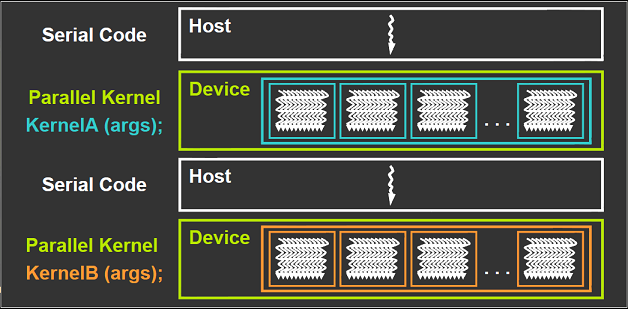
\includegraphics[width=400px]{./images/execution_cuda.png}
  \caption{Ejecución de un programa en CUDA}
  \label{fig:execution_cuda}
\end{figure}

\subsection{Sumar dos vectores}

\subsubsection{Suma secuencial}

Una vez que las funciones para los kernels están definidas en un código fuente, ya no se puede utilizar el compilador de
C tradicional y hay que utilizar un compilador que entienda estas declaraciones adicionales como es el caso de
\texttt{nvcc}.

Como primera aproximación utilizaremos un ejemplo muy sencillo que consiste en sumar las componentes de dos vectores que
es una de las operaciones más sencillas que podemos realizar en computación paralela. Antes de adentrarnos en el código
del \textit{kernel} para la suma de dos vectores, es útil revisar cómo funciona una función de suma de vectores con un
algoritmo secuencial.

\begin{algorithm}
\caption{Suma de dos vectores}
  \begin{algorithmic}[1]
  \Statex \textbf{Define:} vecAdd($a$, $b$)
  \Statex \textbf{Input:} $a = \{a_0, a_1, a_2, \ldots, a_n\}$, $b = \{b_0, b_1, b_2, \ldots, b_n\}$
  \Statex \textbf{Initialization:} $c_0 = 0, c_1 = 0, c_2 = 0, \ldots, c_n = 0$
  \Statex \textbf{Output:} $c_0 = a_0 + b_0, c_1 = a_1 + b_1, c_2 = a_2 + b_2, \ldots, c_n = a_n + b_n$

  \For{$i = 0$ to $n$}
    \State $c_i = a_i + b_i$
  \EndFor
  \end{algorithmic}
\end{algorithm}

\newpage

El mismo algoritmo en C sería algo así:

\begin{lstlisting}[language=C]
  void vecAdd(float* h_A, float* h_B, float* h_C, int n)
  {
    for (int i = 0; i < n; i++) h_C[i] = h_A[i] + h_B[i];
  }
  int main() {
    // Reservamos memoria para h_A, h_B, and h_C // I/O para leer h_A and h_B   (los N elementos cada uno)
    vecAdd(h_A, h_B, h_C, N);
  }
\end{lstlisting}

El código muestra una función que suma dos vectores. Se van a utilizar los prefijos \texttt{h\_} para las variables que
son procesadas por el host y \texttt{d\_} para las variables que son procesadas por el device. En este caso, todas las
variables son procesadas por el host, por lo que sólo se ven las variables \texttt{h\_}.

\subsubsection{Suma paralela}

Una forma sencilla de ejecutar la suma de dos vectores en paralelo es modificar la función \texttt{vecAdd} y mover sus
cálculos a un dispositivo. La forma de hacer esto es:

\begin{algorithm}
\caption{Suma de dos vectores}
  \begin{algorithmic}[1]
  \Statex \textbf{Define:} vecAdd($a$, $b$)
  \Statex \textbf{Input:} $a = \{a_0, a_1, a_2, \ldots, a_n\}$, $b = \{b_0, b_1, b_2, \ldots, b_n\}$
  \Statex \textbf{Initialization:} $c_0 = 0, c_1 = 0, c_2 = 0, \ldots, c_n = 0$
  \Statex \textbf{Output:} $c_0 = a_0 + b_0, c_1 = a_1 + b_1, c_2 = a_2 + b_2, \ldots, c_n = a_n + b_n$

  \comentario{Reservar espacio en la memoria del dispositivo para almacenar copias de los vectores $A$, $B$ y $C$.}
  \Statex reserveMemory $d_A$
  \Statex reserveMemory $d_B$
  \Statex reserveMemory $d_C$

  \comentario{Copiar los vectores desde la memoria del host a la memoria del dispositivo.}
  \Statex $d_A$ = $a$
  \Statex $d_B$ = $b$

  \comentario{Lanzar la ejecución paralela del kernel de suma de vectores en el dispositivo.}
  \Statex launchKernel vecAdd($d_A$, $d_B$, $d_C$)

  \comentario{Copiar el vector suma $C$ desde la memoria del dispositivo a la memoria del host.}
  \Statex $c$ = $d_C$

  \comentario{Liberar los vectores en la memoria del dispositivo.}
  \Statex freeMemory $d_A$
  \Statex freeMemory $d_B$
  \Statex freeMemory $d_C$
\end{algorithmic}
\end{algorithm}

En los sistemas CUDA actuales, los dispositivos son a menudo tarjetas de hardware que vienen con su propia memoria
dinámica de acceso aleatorio (DRAM). Por ejemplo, la NVIDIA GTX1080 viene con hasta 8 GB de DRAM, llamada memoria
global. Usaremos los términos memoria global y memoria del dispositivo de manera intercambiable. Para ejecutar un kernel
en un dispositivo, el programador necesita asignar memoria global en el dispositivo y transferir datos pertinentes desde
la memoria del host a la memoria del dispositivo asignada. Del mismo modo, después de que el kernel haya terminado de
ejecutarse, el programador necesita transferir los resultados desde la memoria del dispositivo a la memoria del host y
liberar la memoria global asignada en el dispositivo.

La figura \ref{fig:host_memory_global_memory.png}, muestra una imagen de alto nivel del modelo de memoria del host y
dispositivo CUDA para que los programadores razonen sobre la asignación de memoria del dispositivo y el movimiento de
datos entre el host y el dispositivo. La memoria global del dispositivo puede ser accedida por el host para transferir
datos hacia y desde el dispositivo, como se ilustra en las flechas bidireccionales entre estas memorias y el host. La
memoria constante puede ser accedida de manera de solo lectura por funciones de dispositivo.

Por ahora sólo importa saber que NVIDIA creó dos funciones nuevas, \texttt{cudaMalloc} y \texttt{cudaFree}. La función
\texttt{cudaMalloc} puede ser llamada desde el código del host para asignar un pedazo de memoria global del dispositivo
para un objeto. El primer parámetro de la función \texttt{cudaMalloc} es la dirección de un puntero que será configurado
para apuntar al objeto asignado. La dirección del puntero debe ser convertida a \texttt{(void **)} porque la función
espera un puntero genérico; la función de asignación de memoria es una función genérica que no está restringida a
ningún tipo particular de objetos. Este parámetro permite a la función \texttt{cudaMalloc} escribir la dirección de la
memoria asignada en el puntero. El segundo parámetro de la función \texttt{cudaMalloc} da el tamaño de los datos a
asignar, en número de bytes. El uso de este segundo parámetro es consistente con el parámetro de tamaño de la función
\texttt{malloc} de C.

Por el otro lado la función \texttt{cudaFree} puede ser llamada desde el código del host para liberar la memoria global
del dispositivo asignada a un objeto. La función \texttt{cudaFree} toma un puntero a la memoria global del dispositivo
que se va a liberar. La función \texttt{cudaFree} no necesita cambiar el contenido del puntero, solo necesita usar el
valor del puntero para devolver la memoria asignada al pool disponible.

En resumidas cuentas el código para crear la memoria en el device sería algo así:

\begin{lstlisting}[language=C]
float *d_A;
int n = 100;                                    // Número de elementos en el vector
cudaMalloc((void **)&d_A, n * sizeof(float));
...
cudaFree(d_A);
\end{lstlisting}

Una vez que el host ha asignado memoria en el dispositivo, puede transferir datos desde la memoria del host a la memoria
del dispositivo utilizando las funciones API de CUDA.

El código para asignar y copiar memoria del host al device y viceversa se da de la siguiente manera:

\begin{lstlisting}[language=C]
void vecAdd(float* h_A, float* h_B, float *h_C, int n) {
  int size = n * sizeof(float);
  float *d_A, *d_B, *d_C;
  cudaMalloc((void **) &d_A, size);
  cudaMemcpy(d_A, h_A, size, cudaMemcpyHostToDevice);
  cudaMalloc((void **) &d_B, size);
  cudaMemcpy(d_B, h_B, size, cudaMemcpyHostToDevice);

  cudaMalloc((void **) &d_C, size);

  // Invocación al kernel... (veremos esto más adelante)

  cudaMemcpy(h_C, d_C, size, cudaMemcpyDeviceToHost);
  cudaFree(d_A);
  cudaFree(d_B);
  cudaFree(d_C);
}
\end{lstlisting}

Notar que \textttt{cudaMemcpyHostToDevice} y \texttt{cudaMemcpyDeviceToHost} son dos constantes que indican la dirección
de la transferencia de memoria. La función \texttt{cudaMemcpy} es una función de la API de CUDA que copia memoria entre
el host y el device. El primer parámetro de la función \texttt{cudaMemcpy} es la dirección de la memoria de destino, el
segundo parámetro es la dirección de la memoria de origen, el tercer parámetro es el tamaño de la memoria a copiar en
bytes, y el cuarto parámetro es una constante que indica la dirección de la transferencia de memoria.

\subsection{Convertir una Imagen a Escala de Grises}

El procesamiento de imágenes es un clásico ejemplo de computación paralela y comenzaremos la introducción a CUDA viendo
un ejemplo de procesamiento de imágenes para ejemplificar los primeros conceptos. En este caso vamos a ver cómo
convertir una imagen a escala de grises.

\begin{tcolorbox}[colback=yellow,colframe=yellow!75!black,arc=0pt,outer arc=0pt]
  \textbf{Threads} \\

  La ejecución de un kernel genera un gran número de threads para explotar el paralelismo de datos. En el caso de la
  conversión de una imagen color a escala de grises cada thread podría ser utilizado para computar un pixel de la imagen
  de salida. En este caso, el número de threads que serán generados por el kernel es igual al número de pixels en la
  imagen. Para imágenes grandes, un gran número de threads serán generados. En la práctica, cada thread puede procesar
  múltiples pixels para eficiencia. Los programadores de CUDA pueden asumir que estos threads toman muy pocos ciclos de
  reloj para ser generados y programados debido al soporte eficiente del hardware. Esto es en contraste con los threads
  tradicionales de la CPU que típicamente toman miles de ciclos de reloj para ser generados y programados.
\end{tcolorbox}

\subsubsection{Representación de una imagen en la computadora}

Antes de comenzar a escribir cualquier tipo de código, tenemos que saber cómo se representa una imagen en la
computadora. Esencialmente una imagen se representa como una matriz de tuplas $(R, G, B)$ donde $R$, $G$ y $B$ son los
valores de los colores (canales) rojo, verde y azul respectivamente. Cada uno de estos canales tiene un valor que va
desde 0 ($0x00$) a 255 ($0xFF$) y representan la intensidad de cada color de un pixel en una imagen. Existen $256^3$
colores posibles y estos colores se representan dentro del triángulo AdobeRGB (ver Figura \ref{fig:adobe_rgb}).

\begin{figure}[H]
  \centering
  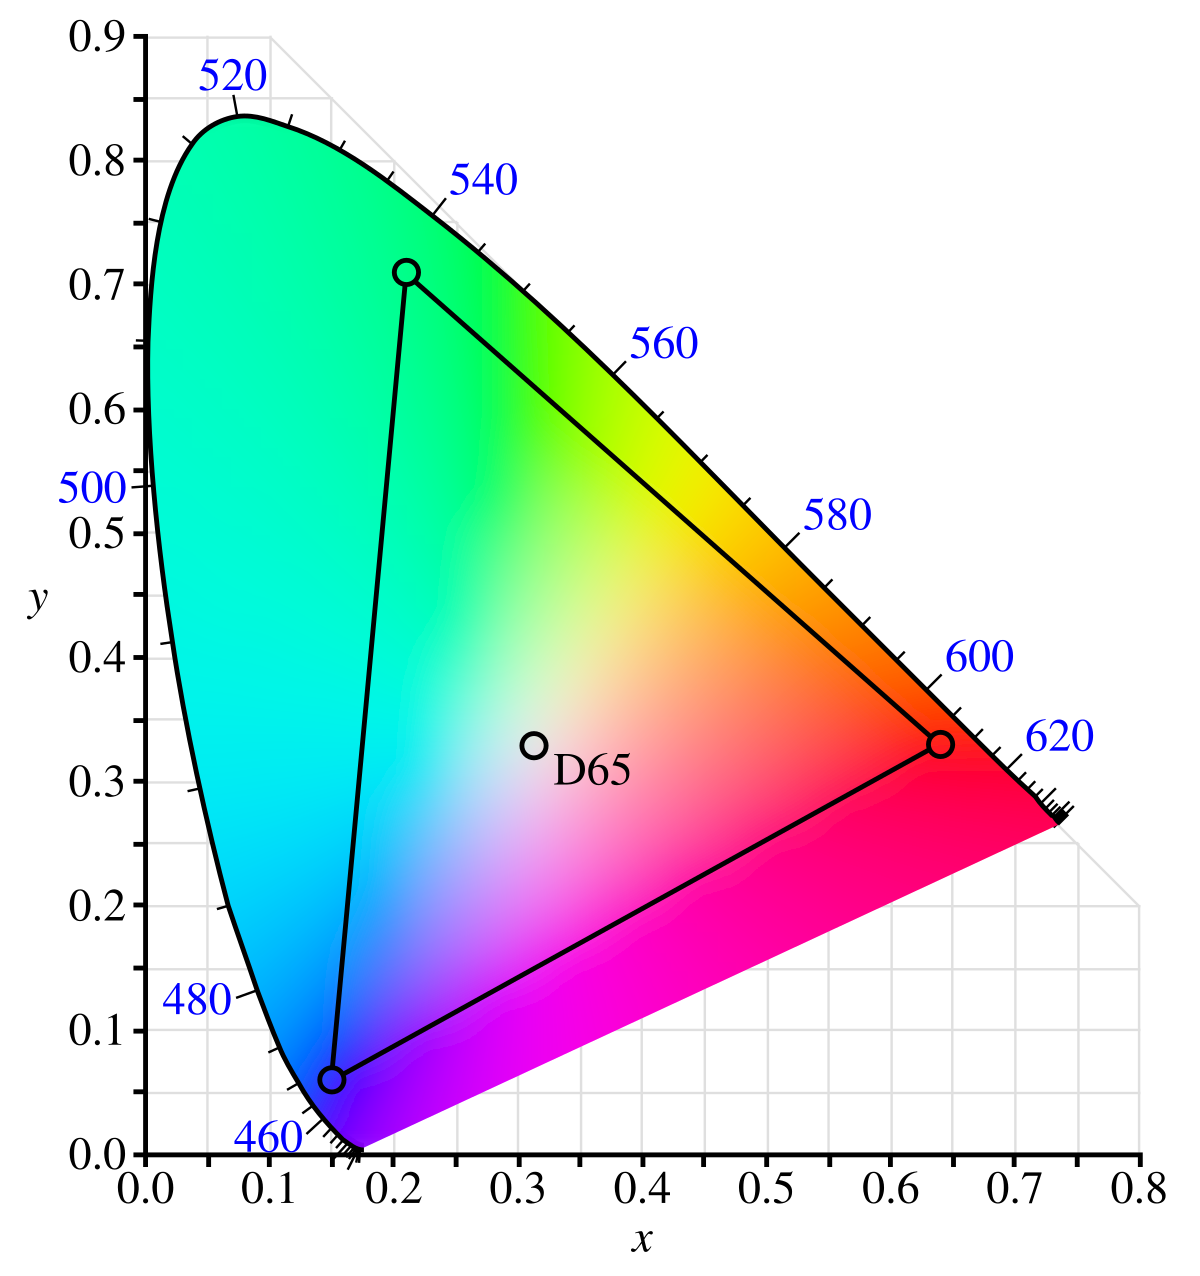
\includegraphics[width=200px]{./images/adobe_rgb.png}
  \caption{Triángulo AdobeRGB}
  \label{fig:adobe_rgb}
\end{figure}

Como dijimos, estos valores de $R$, $G$ y $B$ representan los \textit{canales} y para convertir estos canales a escala
de grises se debe utilizar una fórmula, ya que hay que decidir cuál va a ser la intensidad final del pixel en escala de
grises en la imagen blanco y negro. Esto se hace realizando una combinación lineal de los valores de los canales de
color de alguna manera y, lógicamente hay muchas formas de convertir estos canales a escala de grises. Por ejemplo
podríamos tomar sólo el valor del canal $G$ (verde), haciendo la combinación lineal $pixel_{gris} = R \cdot 0 + G \cdot
1 + B \cdot 0$. De esta manera la imagen sólo se vería representada por ese canal, lo cual no sería muy verídico,
ya que el ojo humano percibe la intensidad de los 3 canales. Como podrán imaginar, hay muchas formas de convertir una
imagen a escala de grises \footnote{¡Podrían probar con diferentes fórmulas y ver cómo se ve la imagen!, hay $256^3$
combinaciones posibles.}, pero hay algunas que son más comunes que otras.

\begin{tcolorbox}[colback=mint,colframe=yellow!75!black,arc=0pt,outer arc=0pt]
  \textbf{Algunas fórmulas comunes para convertir a escala de grises}, son las siguientes: \\

  \begin{itemize}
    \item \textbf{Promedio}: $I = \frac{R + G + B}{3}$
    \item \textbf{Luminosidad}: $I = 0.21R + 0.72G + 0.07B$
    \item \textbf{Desaturación}: $I = \frac{max(R, G, B) + min(R, G, B)}{2}$
  \end{itemize}
\end{tcolorbox}

Para nuestro ejemplo, vamos a usar la fórmula de \textit{luminosidad} para convertir la imagen a escala de grises que es
un promedio pesado de los canales de color, y que representa la percepción humana de la luminosidad, pero como dijimos
no es la única forma y cambiar esta fórmula puede dar diferentes resultados que podrían considerarse como "filtros de
imagen".

\newpage

\vspace{1em}

\printbibliography


\end{document}
